%MEGA MAN X.TEX

\textit{Mega Man X} is born as a spin-off game of the classic Mega Man franchise for the Super Famicon/SNES consoles (later also for PC)  between the 1993 and the 1995\cite{wiki:MMX}. The game takes place one hundred years after the main franchise timeline, in a world where humans and special robots capable of having feelings co-exists and where X, one of those robots, fights the evil Sigma which aims to eliminate humans on order to have a world only for robots.

In the year 2005 a remake for PlayStation Portable was done, upgrading to a 3D graphic close to the precedent title, Mega Man X8. This game (named \textit{Maverick Hunter X }or \mhx in short) had the purpose to re-tell the first game's story with some minor changes such as X relationship with Mavericks and Sigma, which weren't present in the original game. Changes also effected level design, such as Light's capsule positions or Sigma stages, completely different from original ones.

\section[Main plot]{Main plot (X)}
In the year 21XX humans live peacefully with new kind of robots: reploids. Reploids (\ref{dict:reploids}) are particular type of robots with the ability to take autonomous decisions as well as having feelings and sentiments\cite{Xcoll1:Manual_X1}. However sometimes  a reploid' electric brain can undergo  malfunctioning making him act dangerously for nearby humans and others reploids . When this happen the reploid is labeled as ``Maverick'' and has to be stopped, in order to be repaired or disposed, by a special organization created with the exact purpose to stop mavericks: the Maverick Haunters. Leader of the Maverick Haunters is Sigma, one of the most advanced reploid of the time. 

The situation takes a turn when Sigma himself go maverick, declaring war against humanity and recruiting in its rank other maverick haunters, both willing to follow him or threatened by Sigma himself. In order to stop the war X, the main protagonist of the story, decides to joining the fight alongside Zero (a close friend of him) on the highway under attack, but is stopped by Vile,
\begin{wrapfigure}{r}{0.4\linewidth}
	\centering
	
\includegraphics[width=\linewidth]{figures/X1/Highway_screenshot_4.jpg}
	\caption{Vile capturing X.}
\end{wrapfigure} an ex-haunter released by Sigma from prison, in his ride armor. Only the intervention of Zero himself, which force Vile to flee, allow X to escape safely.

The two then decide to split: while Zero goes to locate the enemy fortress, X has to deal with the threat of Sigma's mavericks. As X defeats all the eight mavericks, acquiring in the process new power-ups and strength, he joins Zero who in the meanwhile has located the Sigma fortress flying over the sea. At the entrance however they are immediately confronted with Vile and his ride armor, which first manages to capture Zero (that challenged him in a one-versus-one fight) and subsequently X too. As Vile laughs at his victory, Zero manages to escape from his cage, latches on the ride armor and detonates himself, destroying it but leaving Vile untouched. Seeing his friend's action give X new energy, allowing him to break free too and face Vile, now vulnerable, defeating him in the process. Before going on however X listens to Zero's ultimate words\cite{wiki:MMX_script}. Zero informs X that his auto-repair system cannot handle all damages taken and that X has a power even greater than his own, which makes him capable of face Sigma (eventually Zero also gives X his own Z-buster if he didn't manage to get his own buster upgrade). After that, Zero dies and X proceeds infiltrating Sigma's fortress and his dangers, including re-facing all the previously-defeated mavericks. At the end X arrives at Sigma's place where Sigma is waiting. At first Sigma acts with arrogance, looking surprised that X has managed to reach him with his only forces and claiming he could destroy him without effort. However he decides to leave the pleasure to his pet Velguarder, as he leaves the scene to assist at the fight. After X successfully manages to destroy Velguarder, Sigma changes his mind a little, understanding why Zero placed his trust in X and claiming X could have been an haunter as strong as he was. After that he proceeds to confront X, but gets defeat and his body destroyed, only his head remaining which merges with a giant wolf-based mechaniloid in the room, giving Sigma a new body to fight X. However X succeeds in destroying the new body as well, effectively getting rid of Sigma for good. As Sigma blames X for destroying his dream of a world only for reploids, Sigma himself and the fortress start to explode, forcing X to teleport to the outside. In the end X ponders about the destruction he helped to generate, on the sacrifices made for the victory, and questioning if choosing to fight was the right choice, meditating if another option was possible. As the flying fortress sinks in the ocean, X realizes that he will have to fight more battles before having the answers he needs. 
After the game's credits, it is then revealed that the next battle will not take long before occurring, since a message form Sigma is played, where the maverick states that his spirit is still intact and waiting for a new body to be built for face X again.

\section{Main Plot (\mhx)}
While being for the major part similar to the original plot, \textit{Maverick Haunter X} takes some divergence regarding characters relationship as well as X's background \cite{wiki:MM_MHX}. One of the main divergence point regard X's story prior to the war's start. Next is a summary of \textit{Maverick Haunter X} differences respect \x.

An in-depth background of the war is given, via the ``Day of $\Sigma$""\ref{App:Day_of_Sigma} OVA, explaining how Sigma started his revolution. Here X's background is also changed, now being already a Maverick Haunter (in contrast with the original, where no information are available) serving in the 17th Elite Unit alongside Zero and commanded by Sigma himself. X's haunter rank is B (in contrast to Zero's SA rank) due to his kindness and pacifist spirit, the only ones suspecting of his true potential being again Zero and Sigma. 

Another character with an expanded background is Vile. Here he aims to destroy both X and Sigma, to create his own world, hence following Sigma plans only due the fact some objectives they have match.

Last main difference regards the final portion of the story\cite{wiki:MM_MHX_script}. In fact, while in the original X and Zero immediately face Vile as they enter Sigma fortress, here X first travel through the fortress, facing previous bosses brought back to life, and only at end he meets with Zero and is stopped by Vile. As the main story, however, Vile captures both of them, resulting in Zero sacrificing and X destroying him. Finally, even Sigma has a different attitude regarding X due already suspecting X's great potential. In fact he first tests X by making him fight Velguarder (in contrast with the original game, where Sigma use Velguarder thinking to be sufficient to defeat X) and then challenges X himself, ending in the same way as the original story.	

\section{Main Characters}
\subsection{X}
X(\ref{char:X}) is the first type of a new kind of sentient robot capable of having feeling and take decision of his own developed by Dr. Thomas Light in the year 20XX. Being provided with great power, Dr. Light needed to ensure X's integrity by running a series of test which would have required thirty years to be completed. Unlikely, Dr. Light lifespan didn't allow himself to live longer to complete all tests, so he sealed X in a capsule capable of run the tests in autonomy.


In the year 21XX X's capsule is found by Dr. Cain\ref{cha:Cain} during an archaeological expedition\cite{X:Manual},\cite{wiki:Cain_journal}. Dr. Cain awakes X and, using Light's designs and X help, develop a new kind of robot later called ``Reploids''. X however remains questioning about his place in the world and the future Dr. Light wanted for him. Despite this, when the evil Sigma starts his war against human kind, X is forced to step up and fight in order to restore peace alongside his friend Zero. 


What told until now refers to the original role of X in the \x game. Nevertheless, as stated before, \textit{Maverick Haunter X} re-write X's story by providing a new background for events prior to Sigma's revolt. In this continuity Dr. light seals X away not for testing his integrity, but rather believing the world not to be ready for X's technology and potential. Here Light is firmly convinced that X has a good spirit and that he will use his power to achieve peace\cite{wiki:MM_MHX_X}. Moreover after his awakening X joins the Maverick Haunters (which do not happen in the original story), serving in the 17th Elite Unit, alongside Zero and under the direct command of Sigma. Despite having great potential, however, X's haunter rank is only B (in contrast with the SA rank of Zero) due is what seems to be his lack of decision during battle. In reality this is caused by his pacifist nature, making him reluctant to fight and preventing him to use his real power\cite{Xcoll1:Manual_X1}. Nevertheless, when the evil Sigma starts his war against human kind, X is forced to step up and fight in order to restore peace together with Zero.

\subsection{Zero}
Fighting alongside X against Sigma is Zero\ref{cha:Zero}. In the original \x game, very few information are give regarding Zero, except being a friend of X and the new leader of the Maverick Haunters\cite{X:Manual}, having the highest rank above all haunters which didn't side with Sigma. 
Different is the situation in the \mhx game, where Zero's relationship with X is explained better, the former being close friend and a mentor for X in the 17th Elite Unit, having an SA haunter rank and working under Sigma. Here it is also stated how Zero repel evil with all his strength, fighting merciless against Maverick, Sigma included\cite{Xcoll1:Manual_X1}.  

In any case, Zero story is the same for both games. He first appears at the end of the highway saving X from Vile's grasp, and asking X to take care of Sigma forces while he locates the enemy hideout. Next he's seen at the entrance of Sigma fortress where he suggests to split up, offering to act as decoy to let X sneak inside. Lastly Zero is seen for the last time at the final battle with Vile, where he sacrifices himself to destroy Vile's armor and allow X to defeat him. Finally with his last words he ask X to go and take down Sigma, eventually giving X his own Z-buster, in case X hasn't upgraded it yet.

\section{Game Mechanics}
\textit{Mega Man X}'s gameplay stays faithful to its original series by being a 2D hybrid between a run' n' gun and a platform, where the main protagonist (X in this case) has to clear different stages in order to unlock the final area of the game. Each stage has its own theme, contains a certain number of items to collect (depending on the stage it could be one ore more) which may require other power-ups to be collected first in order to be obtained (typically bosses weapons). Finally at the end of the stage a boss waits, which has to be defeat in order to clear the stage and which will give X a new weapon based on one of his attacks. As the original series all main stages can be accessed in any order and all bosses presents has a ``weak point'' corresponding to a weapon obtained from defeating one another boss first. The ``weak point'' typically consists in a weapon dealing more damage to the boss, but sometimes others effects can occur, such has stunning him or preventing him to do certain actions.

\x introduces however some new mechanics which will later define the series\cite{wiki:X1_features}:
\begin{itemize}
	\item Dash: X, via the boot parts, can dash and move faster, as well as jump higher via a dash-jump.
	\item Wall-jumping: X can jump onto wall in order to climb them or can slide down to descend slowly. He can also dash-jump off to a wall to cover a greater distance.
	\item Armor parts(\ref{X1:Armor}): By finding Light's capsules (four in total) X can be upgraded unlocking new powers which can help the player during the game.
	\item Sub-Weapon charging(\ref{X1:sub_weapon}): via the buster upgrade, X can not only charge his main X-buster, as the main series, but he can also charge his other sub-weapon to increase damage dealt or change their functionalities.
	\item Heart tanks: beside classical Sub-tank X, eight heart tank are also scattered in various stages (one per each). By picking them up X's energy grows by two, starting from 16 up to a maximum of 32\cite{stratwiki:Heart_tank}.
	\item Stage interactions: although a very limited feature, by clearing certain stages, other ones will be effected and change in some portions.
\end{itemize}

\section{Weapons}\label{X1:sub_weapon}
Here is a list of all sub-weapons available in\textit{ Mega Man X}/ \textit{Mega Man Maverick Haunter X} (\cite{MHX:manual},\cite{wiki:X_weapons}):

\subsection{Shotgun Ice}\label{Shotgun_ice}
Shotgun Ice is the weapon obtained by X after defeating Chill Penguin. It absorbs moisture in the air and fires it in crystallized form. If it hits an enemy or a hard surface, it breaks into 5 pieces which ricochet backward and get destroyed if hit another wall or enemy When charged it creates an Chill Penguin-shaped ice platform (only in \x, while in \mhx is only a sharp sled of ice) in similarly to how the boss creates his ice sculpture. X can stand on the platform which will start moving forward shortly after being created. If X creates the platform and then places himself in the same spot where the platform is creating (due the fact that the creation in not immediate) the platform will slightly push X left or right depending of its position, enabling some glitches such as wall clipping(\ref{X1:misc}, only in \x).

\subsection{Electric Spark}\label{Electric_spark}
Electric spark creates high-pressure voltage within the X-Buster and fires it, for a maximum of three shots at time. If the electric spark hits an hard surface, it splits in half, starting to travel up and down along the surface. The charged version of this weapon differs between the original game and his remake. In X1 upon charged X will release two electric columns in front and behind him and which will move in their respective directions, while in \mhx X will generate electricity in all directions. This weapon is acquired upon defeating Spark Mandrill.

\subsection{Rolling Shield}\label{Rolling_shield}
After beating Armored Armadillo, X will gain the Rolling Shield. By using it X spins energy at high speeds within the Buster and launches it	as an energy shot that rolls along the ground. The generated projectile is about the same size as X (half in \mhx) and will roll following the ground until making contact with an enemy or disappear after a while Only in \mhx the shield will absorb any projectile directed toward it, as well as dispose Mets even while hiding\cite{wiki:Rolling_shield}. Upon contact whit a wall, the shield will ricochet once and disappear up hitting a wall again. When charged X will surround himself with an energy field which eliminates any enemy with less than three hit points that hit it, but will disappear upon contact with enemy with more than that life value. In the original game while the charged shield is active X cannot shoot nor change weapon while in game, requiring the player to change weapon from the pause menu and thus making the shield disappear.

\subsection{Homing Torpedo}\label{Homing_torpedo}
When equipping this sub-weapon X gains the ability to fire up to two (three in \mhx)\cite{wiki:Homing_torpedo} torpedoes capable of tracking enemies. As they pick up speed, they home in on the closest enemy and pursue it. When charged X will release a fan of four (six in \mhx) fish-shaped missiles with greater speed and attack power which home better to enemies. This weapon is obtained after defeating Launch Octopus.

\subsection{Boomerang Cutter}\label{Boomerang_cutter}
The Boomerang Cutter is the weapon obtained upon defeating Boomer Kuwanger. It fires a sharp boomerang made from a special metal. If it does not hit an enemy, it returns to its owner. and if it passes an item on its way back, it picks up the	item and delivers it to its own owner (even bringing dropped life/weapon energy from enemies). Up to three cutters can be on screen at the time\cite{wiki:Boomerang_cutter} and their trajectory will depend on the position X was when he fired them: they will arc upwards if X was standing on the ground, while they will arc downwards if X was in the air. If a boomerang successfully return to X without hitting an enemy, it will replenish the energy used to create it. Upon charged X will release four bigger boomerang spiraling out of him diagonally. In \mhx this has been changed with four boomerang of doubled size which will move back and forward in straight line a few times. 

Finally both Flame Mammoth and Launch Octopus, while not being directly weak to Boomerang Cutter, can be heavily damaged when hit with this weapon, the former loosing his trunk and the latter his tentacles, resulting in both being unable to perform certain moves.

\subsection{Chameleon Sting}\label{Chameleon_sting}
The Chameleon Sting, obtained after beating Sting Chameleon, emits a single straightforward laser which than splits into three directions: forward, up-forward, down-forward. In \mhx it instead directly emits three lasers, which can be angled diagonal-up and diagonal-down and are slightly faster. In both games the charged version makes X flash in various colors of the rainbow making him invincible to any damage (besides insta-kill hazards like pits) for a short amount of time. In the original game X cannot switch to any weapon while the invincibility is active, meanwhile in the remake is free to fire both with the current one and any other weapon\cite{wiki:Chameleon_sting}.

\subsection{Storm Tornado}\label{Storm_tornado}
The Storm Tornado turns the X-buster into a high-power fan that blasts opponents with hard-hitting wind, capable of destroying enemies that stand in its path. It shoots an horizontal tornado which stays on the screen for a short amount of time, and then starts moving in the direction X was facing when shot. Due to his length it can hit enemies multiple times, being an effective way to dispose most of them, especially bigger ones.  The \mhx version has its length halved, allowing to shoot it at a faster rate. When charged the Storm Tornado will create a large vortex covering all the screen in high, surrounding X in the original game while exploding from a shot projectile upon hitting a solid surface in the remake.\cite{wiki:Storm_tornado} It is obtained by defeating Storm Eagle.

\subsection{Fire Wave}\label{Fire_wave}
Fire Wave converts the X-buster into a powerful flamethrower, which deals continuous damage to enemies but that cannot be used underwater. Upon pressing the fire button X will start shooting fire from his X buster at a continuous rate draining energy in the process. Once charged X will fire a fireball which creates a wave of fire upon hitting the ground and moves forward for a while. However in order to charge the weapon X must keep firing, draining energy in the process. This weapon is obtained once Flame Mammoth is defeated. 

\section{First Armor}\label{X1:Armor}
While exploring stages X can run into one of the four capsules hidden by Dr. Light. When entering in contact the capsule will open revealing Dr. Light's hologram which will talk to X and give him one of the armor parts\cite{wiki:First_armor}, explaining in the process how it works.
The First Armor is composed by the following parts:
\begin{itemize}
	\item Foot Parts: Namely ``Emergency Acceleration System''\cite{X:Manual} allow X to dash forward, as well as to perform dash-jumps and wall dash-jumps as well as reducing his hitbox's height a little while dashing. Moreover X can destroy specifics blocks by wall-jumping onto them. The capsule containing the foot parts reside right in the middle of the Snow Mountain Stage, being mandatory to take. In \mhx the capsule is instead at the beginning of Factory stage.
	\begin{figure}[h]
		\centering
		
\includegraphics[width=0.5\textwidth]{figures/X1/Armor_foot.jpg}
		\caption{Foot Part capsule location}
	\end{figure}
	
	\item Body Parts: When equipped, X will have all incoming damage reduced by 50\%. It is found in the Forest stage after climbing the wall right before the cave. After defeating RT-55J the capsule will emerge from the ground. Meanwhile \textit{Maverick Haunter X} has moved it in Storm Eagle Stage, requiring the head part to access it.
	
	\item Arm Parts: Allow the X-Buster to be charged up to a third level, and to charge up special weapons. Originally Dr. Light thought this upgrade to be included in the basic X-Buster\cite{X:Manual}, bu he sealed away X when the upgrade was not ready yet, forcing him to turn it into a modification to give to X only later.
	\begin{figure}[h]
		\centering
		
\includegraphics[width=0.5\textwidth]{figures/X1/Flame_armor_2.jpg}
		\caption{Buster Part capsule location}
	\end{figure}

	Despite the capsule itself not being mandatory, the game will in any case give the player the buster upgrade in form of the Z-Buster if the player arrives at facing Vile without having found the capsule. While in \x there are no differences between the Arm Parts and the Z-Buster, in \mhx the former allow to shoot the Spiral Shot, which has the same power of the second-level charged shot but is larger and hit multiple times, while the latter deals more damage against bosses that the previous alternatives. In \textit{Meg Man X} the capsule reside in the Factory stage, requiring a precise dash-jump and the Head Parts to break some blocks in the ceiling, while in the remake it is in the same place the Body Parts was in the original game.
	
	\item Head Parts: When equipped X will gain the ability to break specific blocks with an headbutt, as well as avoid damage from falling rocks in the Forest stage. The capsule is found in the Airport stage, hidden behind an obstacle marked with a flammable warning which can be destroyed simply by shooting at it (it is not required the Fire Wave), and in Flame Mammoth stage in the remake, this time requiring the foot part to break blocks hiding it.
	\begin{figure}[h]
		\centering
		
\includegraphics[width=0.5\textwidth]{figures/X1/Storm_armor_2.jpg}
		\caption{Head Part capsule location}
	\end{figure}
	
	\item Hadoken. While not being technically a component of the First Armor, rather a hidden bonus, this technique is stored too inside a Light's capsule so it is reported here. It allows X to perform the well-know technique from \textit{Street Fighter} by inputting the button combination $\downarrow$ $\searrow$ $\rightarrow$ (with X facing right) + fire button or using the same combination while X is charging and release the charged shot\cite{RTA_wiki:X1}  AND X is at full health. The projectile deals 32 point of damage\cite{wiki:Hadoken} to all enemies, basically one-shotting every non-shielded enemy, bosses included. The only exception is Sigma's final form, and only in the original \textit{Mega Man X}. 
	
	Both in the original game and its remake the capsule is hidden in Armored Armadillo Stage, see \ref{Hadouken} for more information on how unlock it.
\end{itemize}

\section{Useful Techniques}
Here are listed some useful techniques which the game does not explain but can be helpful while playing\cite{RTA_wiki:X1}: %dash shot, wall dash-jump slope jump, boss charged shots
\begin{itemize}
	\item Higher jumps: If the player keeps the jump button down after jumping, the reached height will be greater than the one of a simple jump.
	
	\item Wall dash-jump: With the dash upgrade, X cannot only dash and dash-jump for greater heights, but can also do it off walls, which can be very useful especially in bosses rooms to jump from a side to the other.
	
	\item Dash shots. If X shoots un uncharged shot while dashing, the projectile will deal two points of damage rather than one. This only apply for one projectile on screen at the time, so shooting multiple projectiles while dashing will give the damage boost only to the first, until it collides or exits from screen (see the file videos/dahs\_shot.mp4 for a practical demonstration).
	
	\item Slope jumps: If X jumps while walking down a slope, he will jump higher than normal.
	
	\item Ladder wall jumps: The top every ladder, where it passes through the floor, can also act as a hole where X can wall jump. In order to do so the player has to hold left or right and press jump to leave the ladder an let X start sliding on the edge of the floor. It is also possible to do this in another manner but only for those ladder were the edge can be reached by X by jumping. To activate the ladder jump X must first start climbing the ladder and then drop down immediately, then he will be able to jump and reach the edge and start wall jumping. If X doesn't grab the ladder first, an invisible wall will stop X from grabbing the ledge and will prevent him to start wall jumping.
	
	\item Staring boss fight with a charged shot: If the player enters a boss room while holding down the fire button and a charged shot ready (any level) and release it while X is out of control, X will it shoot immediately as the boss fight starts.
\end{itemize}

\section{Highway Stage}
The Highway Stage (Central HighWay in \textit{Maverick Haunter X}) is the first stage of the game. X arrives here in order to join the fight against Sigma's forces.
%\begin{wrapfigure}{r}{0.4\linewidth}
%	\centering
%	
\includegraphics[width=\linewidth]{figures/X1/Highway_screenshot_1.jpg}
%	\caption{X fighting on the highway.}
%\end{wrapfigure}


 The stage is rather straightforward, having X to travel while eliminating different enemies, while also teaching the player some basic mechanics such as wall-jumping.  The stage can be split into two main sections\cite{stratwiki:HighWay}, the second one having more gaps and pieces of the highway falling as X stands on (recognizable by a darker texture color). In the first section of the highway two sub-bosses are presents in form of \hyperlink{miniboss:Bee_Blader}{Bee Blader}. At the end of the stage X will be attacked by Death Rogumer, which will start sending towards him several \hyperlink{enem:Road_Attackers}{Road Attackers}.

 
 Once some of them have been destroyed, Vile will drop out the airship and start attacking X with his ride armor. Vile is literally invincible, so there is 
 \begin{wrapfigure}[10]{l}{0.4\linewidth}
 	\vspace{-10pt}
 	\centering
 	
\includegraphics[width=0.9\linewidth]{figures/X1/Highway_screenshot_2.jpg}
 	\caption{Road Runner dropping on the highway.}
 \end{wrapfigure}
 no point in fighting. Instead as X drop below a certain amount of energy Vile will start shooting an energy projectile toward X and has soon as it connects, X gets trapped and the fight ends, starting the cutscene with Zero saving X. A common speedrun  technique involve having X getting hurt in order to start the boss fight with low health, which will force Vile to shoot the trapping projectile and then run into it, basically skipping the entire fight.  Attention however has to be made, since Vile will not stop attacking with the armor, which may results in the player being defeated.
 
\begin{figure}[htp]
	\centering
	
\includegraphics[width=0.6\linewidth]{figures/X1/Highway_screenshot_3.jpg}
	\caption{Vile preparing to face X}
\end{figure}
This stage contains following enemies\cite{wiki:Highway}:
\begin{itemize}
	\item \hyperlink{enem:Ball_De_Voux}{Ball De Voux }
	\item \hyperlink{enem:Bomb_Been}{Bomb Been }
	\item \hyperlink{enem:Crusher}{Crusher }
	\item \hyperlink{enem:Gun_Volt}{Gun Volt}
	\item \hyperlink{enem:Jamminger}{Jamminger}
	\item \hyperlink{enem:Road_Attackers}{Road Attackers }
	\item \hyperlink{enem:Spiky}{Spiky }
	\item \hyperlink{miniboss:Bee_Blader}{Bee Blader }
\end{itemize}

\begin{figure}[htp]
	\centering
	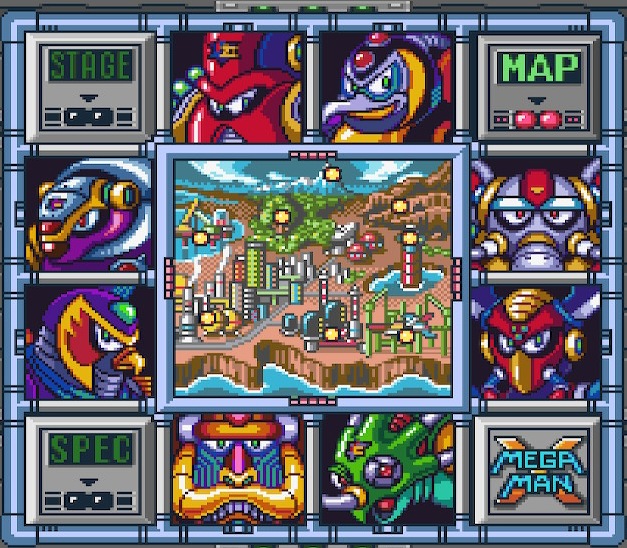
\includegraphics[width=0.6\linewidth]{figures/X1/Full_map.png}
	\caption{Full map with Bosses and their locations}
\end{figure}
 
 
 
\section{Ocean}
The \textit{Ocean stage} (later renamed Subterranean Base in \mhx) is where Launch Octopus hides himself. Here X starts from the shoreline to immerse short after the beginning of the level. Once underwater X will jump higher than normal which, combined with the dash-jump and the beginning of the level being placed on top of a cliff, making the player capable of skipping a good portion of the first part of the underwater scenario\cite{stratwiki:Ocean}. Various fish-based enemies are present, but main difficulties of the sub-bosses the stage has, being three plus an optional one. In the first part main difficulties are given by spiked pit which X has to jump and from where Sea Attacker will spawn in group of three, interrupting X's jump and making him fall into the pit, and from the two Angler sub bosses, the second one being particular dangerous, since the floor has two spiked pits and the Angler will keep using his vacuum attack to push/pull X into them. Here the best strategy consists in stay at the leftmost platform and keep shooting, dashing to the right once it start pulling and shooting while it pushes X. Other than that Anglers will also shoot X four serpent-shaped harpoon which will move horizontally and then fall onto X when they're above him. Finally Anglers will rarely shoot a beam of light from their lamp, which can also be destroyed. After passing the second sub-boss the second part of the stage begins. Here spiked gaps are rarer (although still present) and whirlpools will start to appear at regular intervals and in specific positions. Those whirlpools can be used to propel X up to the ocean's surface. Proceeding in the stage bombs will start dropping from above, fired by a Cruiziler enemy. X can either climb a whirlpool to get onto it and destroy its core, making it sink and stop it from shooting bombs, or avoiding it and proceed in the level. Once passed falling bombs, X will find himself into an arena filled with sand. Here an Utuboros will start attacking him, rising from the sand, than swimming for a while and then immerse again in the sand. It is invincible for most of its body (which X can stand on), only the head and tail being vulnerable. Although its weakness is considered to be the Boomerang Cutter, due to lack of invincibility frame a single Storm Tornado fired behind its head will destroy him in one shot\cite{wiki:Utuboros}. After this other sub-boss X will have go on only for a little before finding himself in front of the boss door.
Following enemies are present in the stage\cite{wiki:Ocean}:
\begin{itemize}
	\item \hyperlink{enem:Amenhopper}{Amenhopper}
	\item \hyperlink{miniboss:Anglerge}{Anglerge}
	\item \hyperlink{enem:Gulpfer}{Gulpfer }
	\item \hyperlink{enem:Cruiziler}{Cruiziler}
	\item \hyperlink{enem:Mega_Tortoise}{Mega Tortoise }
	\item \hyperlink{enem:Sea_Attacker}{Sea Attacker}
	\item \hyperlink{enem:Sky_Claw}{Sky Claw }
	\item \hyperlink{miniboss:Utuboros}{Utuboros}
\end{itemize}

\subsection{Heart Tank}
\begin{figure}[h]
	\centering
	\begin{subfigure}{0.4\textwidth}
		\centering
		
\includegraphics[width=\linewidth]{figures/X1/Octopus_heart_1.jpg}
		\caption{}
	\end{subfigure}
	\begin{subfigure}{0.4\textwidth}
		\centering
		
\includegraphics[width=\linewidth]{figures/X1/Octopus_heart_2.jpg}
		\caption{}
	\end{subfigure}\\
	\begin{subfigure}{0.4\textwidth}
		\centering
		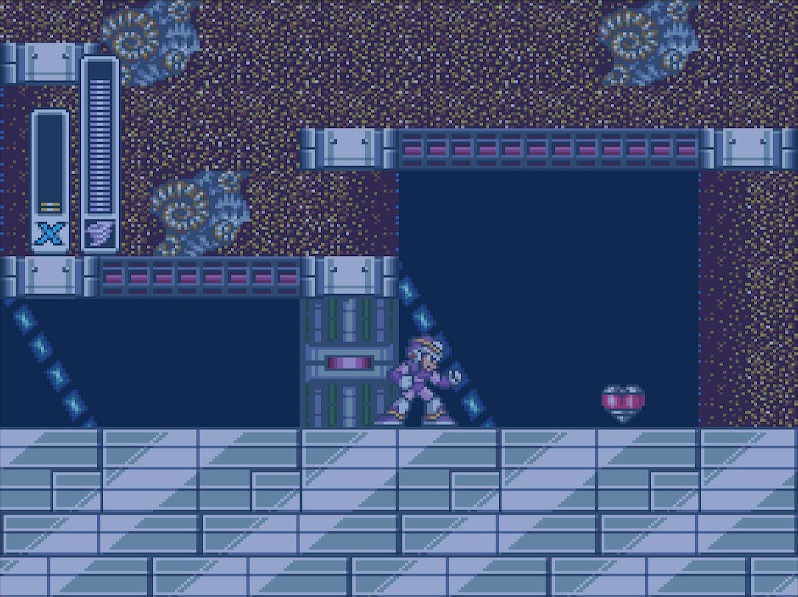
\includegraphics[width=\linewidth]{figures/X1/Octopus_heart_3.jpg}
		\caption{}
	\end{subfigure}
	\caption{(a)Via whirlpool the player can reach the Cruizer on ocean's surface,(b) When destroyed the ship will fall down, breaking the ocean floor and opening a new path,(c) One destroyed the Utuboros inside the cave, a room will open with the Heart Tank inside}
\end{figure}
This stage only has an heart tank has its collectible. In order to get it the player musts first destroy the Cruizer by reaching the ocean's surface via a whirlpool,climb on it and then shoot at its blue core, avoiding the Sky Claws which the ship will spawn. Once destroyed the Cruizer will sink and will destroy the ocean floor, revealing an hidden portion with a large room filled with spiked gaps on the ground. Here another Utuboros (technically the first since the other reside later in the level) must be defeated, in order to open the door which leads to an Heart Tank. After that X must exit from where he entered and climb the wall where the ship fall in order to return to the main path.

\subsection{Launch Octopus}\label{boss:Launch_octopus}
Launch Octopus, the ``\textit{General of the Deep Sea}''\cite{book:MMX_Complete_art} was a Maverick Haunter of the 6th fleet armada before joining Sigma's rebellion and setting his base in the dept of the Ocean, in order to attack marine cities with his army of mechaniloids and to cut off shipping routes. In \x he joins Sigma due the fact he shares the dream of a world only for reploids, having always had doubt on protecting humans, while in \mhx he is pictured military tactician which want to achieve beauty in combat, considering himself an unappreciated artist of underwater fighting. Only Sigma understand his art, making Launch Octopus side with him\cite{wiki:MM_MHX_script}.

\begin{figure}[h]
	\centering
	\begin{subfigure}{0.5\textwidth}
		\centering
		
\includegraphics[width=\linewidth]{figures/X1/Octopus_missile.jpg}
		\caption{}
	\end{subfigure}
	\begin{subfigure}{0.49\textwidth}
		\centering
		
\includegraphics[width=\linewidth]{figures/X1/Octopus_piranha.jpg}
		\caption{}
	\end{subfigure}\\
%	\begin{subfigure}{0.5\textwidth}
%		\centering
%		
\includegraphics[width=\linewidth]{figures/X1/Octopus_vortex.jpg}
%		\caption{}
%	\end{subfigure}
	\begin{subfigure}{0.5\textwidth}
			\centering
			
\includegraphics[width=0.5\linewidth]{figures/X1/Octopus_drain.jpg}
			\caption{}
	\end{subfigure}
%	\begin{subfigure}{0.5\textwidth}
%		\centering
%		
\includegraphics[width=\linewidth]{figures/X1/Octopus_cut.jpg}
%		\caption{}
%	\end{subfigure}
	
	\caption{Launch Octopus attack: (a) Homing Torpedo, (b) Charged Homing Torpedo, (c) Vortex and (d) Draining. In (e) it is possible to see his tentacle cut off}
\end{figure}

In battle Octopus has two main techniques: Homing torpedo and Energy Drain. In reality he has a third technique, which consists in firing what can be considered a charged version of his Homing Torpedo. Both his types of missiles can be destroyed by shooting at them. Launch Octopus will always start the boss fight with a barrage of homing missile, to than switch to one of the other two weapons he has. Just like X, Octopus can fire a charged version of his homing missiles, which are piranha-shaped and homes much faster than their counterpart. Finally he has his Energy Drain attack. When performing this Octopus will first swim on top of the arena, either left or right, and then start spinning to create a whirlpool to suck X in. If he succeed he will start draining X energy to replenish his own, prolonging the fight. Octopus main weakness is the Rolling Shield, which deals him extra damage but can be hard to hit, due Octopus high mobility and the shield colliding with his missiles instead. However Octopus can be also heavily damaged by the Boomerang Cutter, which in three hits will sever his tentacles blocking him to perform his Energy Drain attack. 

Officially\cite{wayback:X_resources} Launch Octopus is 232 cm tall and 182 Kg heavy, in contrast with in-game information\cite{wiki:Launch_Octopus} which show a weight value smaller than the actual one (see fig \ref{Octopus_specs}).

One Launch Octopus has been defeated X will gain the Homing Torpedo(\ref{Homing_torpedo}) weapon, as well as cause a flood in the Forest Stage, making water appear near the beginning of the stage.
\begin{figure}[htp]
	\centering
	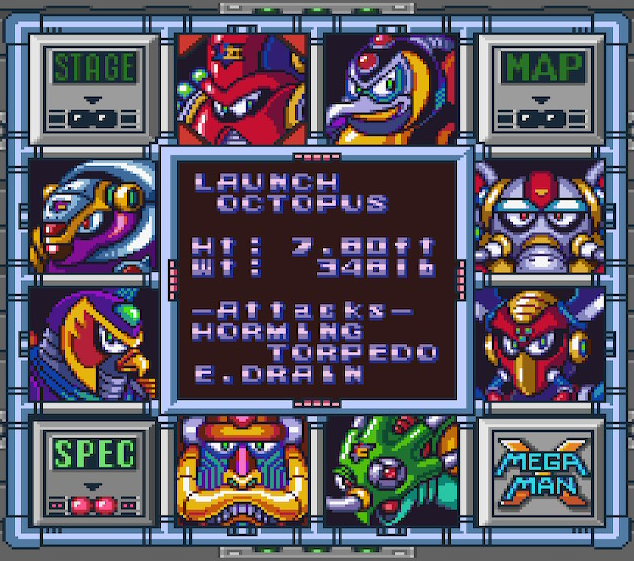
\includegraphics[width=0.6\linewidth]{figures/X1/Launch_octopus_specs.png}
	\caption{Launch Octopus specifications according to X1}
	\label{Octopus_specs}
\end{figure}

\section{Snow Mountain}
\textit{Snow Mountain}(\textit{Abandoned Missile Base in \mhx}) is probably the first stage most people go when starting the game, due to its low level of danger it contains\cite{stratwiki:Snow_mountain}, as for having inside the most useful upgrade X get can get, the Foot Parts. The stage, as the name states, takes place in a snow-covered mountain which X has to climb to get to the boss. The stage is divided into three main areas. The first area is where X starts and consists in a path that brings him inside a cave through a series of enemies. Once inside the cave (the second area) X has first to climb it by following a zig-zag path while also avoiding enemies which drop from higher level, and then to surpass some iced platform separated by pits until he reaches the end of the cave. In the third area X is again on the outside. Here he can take a Ride Armor and proceed for a while. With the armor X can also destroy the igloo he finds and that would otherwise start spawning enemies. Passed the first igloo a choice can be made: to keep the Ride Armor and enter the small cave which comes next, where it is request to jump some gaps using the armor while also face another enemy Ride Armor, or use the armor to reach the top of the cave (jumping out of the armor to gain extra lift), basically skipping the lower portion. After that section X meets a tall wall which the armor cannot surpass, forcing him to leave it behind. Here he has to following a path full of slopes, gaps and Snow Shooters, which will throw snowballs at him and that become bigger the longer they roll on the snowy ground. After passing these enemies, the player will reach the boss door.

The stage contains following enemies\cite{wiki:Snow_mountain}:
\begin{itemize}
	\item \hyperlink{enem:Armor_Soldier}{Armor Soldier} (with Ride Armor)
	\item \hyperlink{enem:Axe_Max}{Axe Max}
	\item \hyperlink{enem:Bat_Bone}{Bat Bone}
	\item \hyperlink{enem:Bomb_Been}{Bomb Been}
	\item \hyperlink{enem:Flammingle}{Flammingle}
	\item \hyperlink{enem:Jamminger}{Jamminger }
	\item \hyperlink{enem:Ray_Bit}{Ray Bit}
	\item \hyperlink{enem:Snow_Shooter}{Snow Shooter}
	\item \hyperlink{enem:Spiky}{Spiky}
	\item \hyperlink{enem:Tombot}{Tombot}
\end{itemize}
\subsection{Foot Parts}\label{X:Foot_Parts}
This stage contains the Armor capsule for the Foot Parts, which allows X to dash, moving faster, perform dash-jumps and wall dash-jumps and alse reducing a little the height of this hitbox. The capsule is found on directly path after having climbed the first part of the cave. Since it is right in the middle of the path it is not avoidable, making it the only mandatory capsule of the entire series.
	\begin{figure}[h]
	\centering
	
\includegraphics[width=0.5\textwidth]{figures/X1/Armor_foot.jpg}
	\caption{Foot Part capsule location}
\end{figure}
\subsection{Heart Tank}\label{Penguin:heart_tank}
The Heart Tank of this stage is hidden in the last igloo X meet before facing the section with snow balls. To reach it X has to jump using the Ride Armor. Right after the first igloo there is a light blue column, right before the cave with the enemy Ride Armor. From the top of the column the player has to jump with the armor and, once reached the maximum height, jump out of it in order to reach the wall which brings to the upper path. Here two other igloo are found which can be destroyed, now that the armor is gone, by using the Fire Wave weapon. In particular the last one contains the searched Heart Tank.

\subsection{Chill Penguin}\label{boss:Chill_Penguin}
The ``\textit{Glacial Emperor}''\cite{book:MMX_Complete_art}), better known as Chill Penguin was a reploid of the 13th Polar Division, specifically designed for operating in polar environments also tanks to his small-size body. However due to the long permanence in the South Pole, away from civilization, Chill Penguin grown tired of his mission, seeking a way to get away from there. Sigma's rebellion give him exactly what he needed to get away, allowing him to escape and join Sigma in his fight. There are however some differences in how his story is told between \x and \textit{Maverick Haunter X}. In the former, after Sigma starts his revolt, Chill Penguin autonomously eliminated his own commander and escaped to join Sigma while also returning to the civilization\cite{Xcoll1:Manual_X1}. Once arrived Chill Penguin seized a mountain base in order to crush nearby cities using avalanches. Meanwhile in the remake it is Sigma himself which took away Chill Penguin from the South Pole by making him join the 17th division together with X and Zero, even before the revolution's beginning\cite{MHX:manual}. Later, while facing X, Chill Penguin revealed that, beside leaving the South Pole, he also joined the revolt due the payment Sigma gave him\cite{wiki:MMX_script}. Another minor difference with the original version is that, in the remake, Chill Penguin seized an abandoned missile base, hinting his purpose was to use it to attack the cities. He's known to be a belligerent, rowdy (sometimes even warped) individual, while also having trouble with his partner Flame Mammoth (\ref{boss:Flame_mammoth}) due his jealously of Mammoth size and the latter attitude of bullying smaller reploids.


\begin{figure}[h]
	\centering
	\begin{subfigure}{0.5\textwidth}
		\centering
		
\includegraphics[width=\linewidth]{figures/X1/Chill_shot.jpg}
		\caption{}
	\end{subfigure}
	\begin{subfigure}{0.49\textwidth}
		\centering
		
\includegraphics[width=\linewidth]{figures/X1/Chill_frozen.jpg}
		\caption{}
	\end{subfigure}\\
	\begin{subfigure}{0.5\textwidth}
		\centering
		
\includegraphics[width=\linewidth]{figures/X1/Chill_shatter.jpg}
		\caption{}
	\end{subfigure}
	\begin{subfigure}{0.49\textwidth}
		\centering
		
\includegraphics[width=\linewidth]{figures/X1/Chill_slide.jpg}
		\caption{}
	\end{subfigure}\\
	\begin{subfigure}{0.4\textwidth}
		\centering
		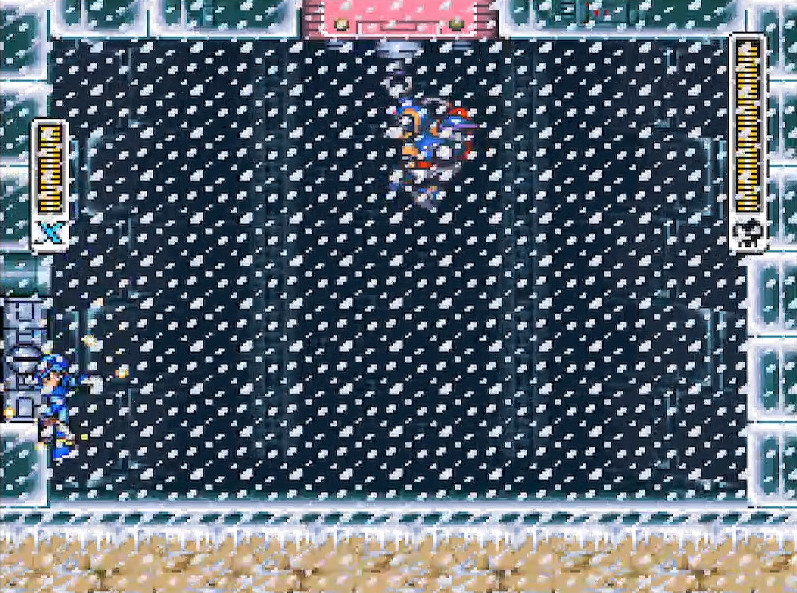
\includegraphics[width=\linewidth]{figures/X1/Chill_blizzard.jpg}
		\caption{}
		
	\end{subfigure}
	%	\begin{minipage}{0.49\textwidth}
	%		\centering
	%		
\includegraphics[width=\linewidth]{figures/X1/Chill_burn.jpg}
	%	\end{minipage}
	\caption{Chill Penguin's attack: (a) Shotgun Ice, (b) X frozen near the two ice statues, (c) Chill Penguin's shotgun ice stopped by his own statues, (d) Chill Penguin slide attack and (e) blizzard attack.}
	
\end{figure}
Chill Penguin is often considered the easiest boss of the game and the first one a player must face due the simplicity of avoiding his attacks, also thanks to the Foot Parts the stage give to the player. He has four main attack which will perform at random\cite{wiki:Chill_Penguin}. When he use his Shotgun Ice, Chill Penguin will shot four frozen projectiles which travel in a straight line, although some of them  can fall off and slide on the ground, which shatter upon contact with a wall but can nullify X shot if the two met. Other times instead of his projectiles he will emit snow which will create two penguin-shaped ice sculpture and, if X is in range, will also freeze him in place. Sculptures act both as obstacles (X takes damage if he makes contact with them) and as cover since both X and Chill Penguin projectiles will be stopped by them.However X shots can damage and eventually break them. In some occasion Chill Penguin will leap in the air and grab the hook on the ceiling, unleashing a blizzard which will push X and the statues (if present) against a wall. When the sculpture hit a wall they shatter. Finally he can also slide on the floor for a while, turning immediately in case he hits a wall. While in this state he is invincible, but will also get rid the sculpture he creates.  As it is possible to see, Chill Penguins attacks only cover the low part of the arena, meaning the best strategy to fight him consist in staying on the higher part via continuous wall-jumps, only dropping to hit him when possible. Attention however must be made, since sometimes Chill Penguin will perform a high jump toward X position which can hit him even if he's  in the high corner of the room. Beside that he can be hit at any times, even when grabbing the hook, beside when sliding. He's weakness is the Fire Wave, which will burn and stun him for a while, but it has no other particular effect.


After defeating him X will gain the Shotgun Ice(\ref{Shotgun_ice}) weapon as well as freezing the lava in the Factory Stage, considerably reducing the danger level of the stage.

Chill Penguin is 163 cm tall and 108 Kg heavy, despite the information screen on the game report different(\ref{Penguin_specs}).

\begin{figure}[h]
	\centering
	
\includegraphics[width=0.5\linewidth]{figures/X1/Chill_penguin_specs.jpg}
	\caption{Chill Penguin specifications according to X1.}
	\label{Penguin_specs}
\end{figure}

\section{Gallery}
The Gallery Stage (or Energy Mines Ruins in \mhx) is the stage controlled by Armored Armadillo. Peculiarity of this level are its mine cart which X can stand and, as soon as he does it, they start moving following the track, increasing their speed as they keep going and destroying all enemies that enter in contact with it. Hoever the player must be careful, as all the carts end their run into pits, bringing X down with them if he doesn't jump off at the right moment. This stage is also famous for containing the secret Light's capsule which teach X the Hadouken technique, as well as being the best place to farm health capsule and lives.

The stage itself is rather simple. Immediately at the beginning a mine cart is present which brings the player forward in the level while also taking care of enemies, but that end its ride when it comes across a series of gaps, one of which it cannot jump and falls into. For that moment the player must have dismount from the cart. After this sequence only few small gaps and some enemies separate X from the next section, which begin when he has to fall off a long pit in the ground. Here as he touches the floor a Mole Borer will destroy the left wall and start chasing X. It is invincible and its roller can insta-kill X if he touches it. Here only two solutions are possible: the first one is to escape to the right, continuing in the level; the second one is, as soon as X reaches the ground, wall jump immediately to the left before the Mole Borer breaks the wall and then jump down, following it from behind (while also gaining acces to the sub tank). In both cases the player has to go right to continue, followed by the mechaniloid (which will eventually crash and explode) or not. After this section another mine cart waits, which will bring the player deeper in the level and, again, end its ride into a pit. Just like the before after this part another large hole in the ground is present and X has to fall off to proceed, meeting another Mole Borer once he lands. This time however he will land behind it, avoiding another chase and, on the other hand, allow the mechanilod to create a passage for the player, until it crashes and explodes again (the player may also want to destroy it since while going it also destroys the access to the heart tank) . Here there is the final cart X has to take to proceed. This mine cart brings X through many enemies until it reaches an opening on the mountain and flies off over a huge gap, impossible for X to jump. Once in the air the player must jump off the cart in order to land on the other side of the pit (or grab the wall if high enough), where the boss door is. While riding in the final parts a group of mechanical birds enemies will start spawning and fly alongside X. Since they fly the cart cannot destroy them, but X will have to, since they can mess up the final jump by hitting him and making him fall into the pit.

Following enemies are present in the stage\cite{wiki:Gallery}
\begin{itemize}
	\item \hyperlink{enem:Bat_Bone}{Bat Bone} 
	\item \hyperlink{enem:Batton_M-501}{Batton M-501} 
	\item \hyperlink{enem:Dig_Labour}{Dig Labour} 
	\item \hyperlink{enem:Flammingle}{Flammingle} 
	\item \hyperlink{enem:Metal_Wing}{Metal Wing} 
	\item \hyperlink{enem:Metall_C-15}{Metall C-15} 
	\item \hyperlink{miniboss:Mole_Borer}{Mole Borer}
	\item \hyperlink{enem:Spiky}{Spiky}
\end{itemize}

\subsection{Sub Tank}
The Sub Tank is located where the first Mole Borer spawn. In order to get it the player has, once arrived to the firs big gap in the ground, jump into it and then immediately wall-jump to the left, in order to let the Mole Borer break the wall and go right passing under X. Once it is passed, the player can safely jump off and go left to find the sub tank where the Mole Borer originally was. 

\subsection{Heart Tank}
The heart tank is located near where the second Mole Borer is found. Once the X jumps off the gap he has to chase the mechaniloid and destroy it in time, since as he proceed it destroy the walls which allow to access the Heart Tank. To do this the Fire Wave weapon is suggested, since it deals massive amount of damage to it in a short span. 

\subsection{Hadouken}\label{Hadouken}
The Hadouken is the last upgrade X can get before facing finals stages. The capsule containing it can be unlocked only of the player has managed to collect every other upgrade in the game: eight Heart Tanks, four Sub-Tank, four armor capsule and all the weapon from bosses. Next the player has to travel trough the gallery stage and reach the top of the ledge above the boss door at least three time after defeating Armored Armadillo, all of them at full health. At the fourth time, near the usual health drop, there will also be the secret capsule.

The best way to make the capsule spawn is as follow: As the stage begin, the player has to travel the level (by walking or on the mine cart) unit it reaches the zone where a single Batton M-501 drops from the roof (near the first slope). Here he should farm lives by continuing killing that enemy (which has a increased drop rate for them)  and making it respawn (it is suggest to use a charged Rolling Shield as it destroy it in one hit). After having accumulated enough lives (at leas five) the player can proceed in the level until the last mine cart is reached, making sure to be at full health by this point. Here X has first to release a charged Sting Chameleon and immediately after ride the cart until over the pit, where he should jump off and grab the ledge over the boss door, reaching the top of if. As X reaches it, he has to jump into the pit, loosing a life and respawning at the last checkpoint (before the second Mole Borer). From here the player has to repeat this procedure for other three times until, at the  fourth one, the capsule will be there. In the remake the capsule does not require multiple travel through the stage, being available immediately.

Once opened the capsule will reveal Dr. Light wearing robe similar to Ryu's one from the Street Fighter series, which will ask X to step into the capsule to teach him the technique. In the Japanese  script of the game\cite{wordpress:X_japanese_script} Light states that he trained under the nearby waterfall a lot to learn it, and that he will now teach it to X who can learn it, as stated again by Light himself in the \mhx remake during the same occasion, due to him having a nearly-human soul.

\subsection{Armored Armadillo}\label{boss:Armored_Armadillo}
Armored Armadillo was the commander in charge of the 8th armored force, as well as a soldier loyal to his superior, Sigma. Once the latter started his revolt, Armored Armadillo blindly followed his orders, occupying a mine to extract raw materials from which Sigma aims to create weapons for his plans.

Faithful to his name and title (``\textit{Armored Warrior}''\cite{book:MMX_Complete_art}) Armored Armadillo fights by using his impenetrable armor both as a shield to deflect X shots and as a weapon to crush him while rolling. When guarding Armadillo is invincible to attacks X performs and, moreover, he can also absorb and re-release charged shot which X fired at him. His main attack is the Rolling Shield, which see him turning into a ball and start bouncing off the walls of the arena while also being immune to any attack. Finally he can sometimes take out the cannon hidden in his forehead and start shooting a sequence of rapid bullet in a straight line. The main difficulty in facing Armored Armadillo is given mainly by the few time he leaves open himself to hits before turning invincible and start attacking again. To solve this problem his weak point comes in play. Armored Armadillo is in fact extremely weak to the Electric Spark since not only this weapon deals him more damage than others but it also can remove his plating. Once deprived of his armor, Armadillo won't be able to guard himself anymore and will also lost his invincibility while rolling, basically making the fight much easier for the player to manage.

Upon beating Armored Armadillo X gains the Rolling Shield weapon(\ref{Rolling_shield}), but no other effects take place in other stages.

According information give, Armored Armadillo is 194 cm tall and 232 kg heavy, while in-game information report him slightly smaller and lighter(\ref{Armadillo_specs}).

\begin{figure}[h]
	\centering
	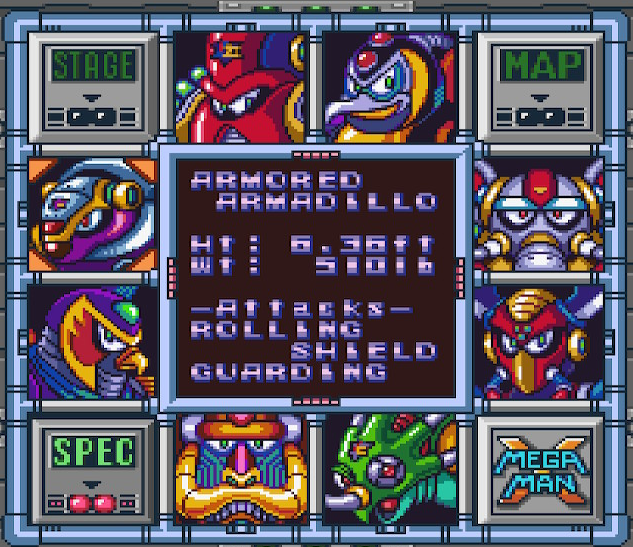
\includegraphics[width=0.5\linewidth]{figures/X1/Armored_armadillo_specs.png}
	\caption{Armored Armadillo specifications according to X1.}
	\label{Armadillo_specs}
\end{figure}
\section{Factory} 
The \textit{Factory Stage}(\textit{Prototype Weapons Plant} in \mhx)  is probably one of the most difficult stage among the eight, due to the high number of danger X can met and that can kill him instantly. The level takes place inside a factory which has been designated to weapons production, as the numerous conveyor belts, presses, and molten metal suggest and that X must face before reaching the boss. However if X manages to defeat Chill Penguin before facing this level, he will found the metal frozen solid, reducing considerably the danger level of the area, as he can stands on it whether he falls from a conveyor belt.
\begin{figure}[h]
	\centering
	\begin{subfigure}{0.49\textwidth}
		\centering
		
\includegraphics[width=\linewidth]{figures/X1/Flame_fire.jpg}
		\caption{}
	\end{subfigure}
	\begin{subfigure}{0.49\textwidth}
		\centering
		
\includegraphics[width=\linewidth]{figures/X1/Flame_frozen.jpg}
		\caption{}
	\end{subfigure}\\
	\caption{Factory Stage before (a) and after (b)  defeating Chill Penguin}
\end{figure}

The stage can be divided into four parts. At the beginning two sets of conveyor belt are present over molten metal which will try to obstacle his movement, together with  \hyperlink{enem:Scrap_Robo}{Scrap Robos} which will keep spawning on them and that will try attack X by crawling at him or by shooting lasers. At the end of this section X has to jump off a hole into the ground which brings him deeper into the factory. The next section is where all the level power-up are concentrated. I consists in a single big room, again on top of molten metal, without conveyor belts but with multiple platform at different heights from which enemies will attack X throwing down their pickaxes. The main danger here is given by the trajectory of the pickaxes since, being parabolic, allow them to be throw safely from upper levels (eventually even from off-screen) without giving X the chance to fire back until he reaches the same platform the enemy stands on. Reached the exit of this part on the top right of the room, another section with conveyor belts and Scrap Robo is present, this time with the addition of presses which insta-kill X if he gets caught. Finally the last part of the stage sees X walking on pipes. Here dangers comes from molter iron dripping from pipes, although it only damages X,  \hyperlink{enem:Rolling_Gabyoall}{Rolling Gabyoalls} which move along pipes while also flipping up and down and finally \hyperlink{enem:Hoganmer}{Hoganmers}, enemies which can bi hit only when attacking (as they lower their shield) or by attacking them from behind. In this section some ladders are present, but their only purpose it to create side-paths to skip enemies, but their utility is questionable. At the end of this section there is the boss door which leads to Flame Mammoth.

These enemies appears in this stage\cite{wiki:Factory}:
\begin{itemize}
	\item \hyperlink{enem:Dig_Labour}{Dig Labour} 
	\item \hyperlink{enem:Hoganmer}{Hoganmer}
	\item \hyperlink{enem:Metall_C-15}{Metall C-15}
	\item \hyperlink{enem:Scrap_Robo}{Scrap Robo}
	\item \hyperlink{enem:Sky_Claw}{Sky Claw}
	\item \hyperlink{enem:Rolling_Gabyoall}{Rolling Gabyoall}
\end{itemize}

\subsection{Arm Parts}
At the entrance of the big room the player will notice some blocks on the roof which can be broke with the Head parts. In order to do so the player will have to dash-jump to the left from the very end of the first platform in order to make X destroy rightmost block which will allow him to wall-jump on the remaining one. Once X has started wall jumping the player has to keep going, in order to climb while destroying remaining blocks and then to access the capsule with the Arm Parts. It is a very precise jump, so many tries can be needed. Furthermore it is possible that X can destroy the block but not starting to wall jump, falling on the ground. This complicates the situation, since the jump now is even more difficult, but still doable, requiring enough precision to make X land on the remaining block at sufficient height to start a wall jump. If for some reasons the player destroy the second block too the climb became impossible and the player has to kill himself to reset the area.
\begin{figure}[h]
	\centering
	\begin{subfigure}{0.4\textwidth}
		\centering
		
\includegraphics[width=\linewidth]{figures/X1/Flame_armor_1.jpg}
		\caption{}
	\end{subfigure}
	\begin{subfigure}{0.5\textwidth}
		\centering
		
\includegraphics[width=\linewidth]{figures/X1/Flame_armor_2.jpg}
		\caption{}
	\end{subfigure}\\
	\caption{Buster upgrade position: a dash-jump is required from (a) to to start wall-jumping and break the ceiling to reach (b).}
\end{figure}

\subsection{Sub Tank}
In the big room, while going to the top-right brings to the exits, going to the top-left corner will bring the player to the sub tank. To obtain it the player has first to reach the highest platform (the one with a life up) and then dash-jump to the left to reach the wall and climb it. While climbing X will reach a part of the wall made of block breakable with the Foot Parts. Behind these blocks there is a small path with the sub tank in it.
\begin{figure}[h]
	\centering
	
\includegraphics[width=0.35\textwidth]{figures/X1/Flame_tank.jpg}
	\caption{Flame Mammoth's Sub Tank}
\end{figure}



\subsection{Heart Tank}
As the previous power-ups, the Heart Tank too is ``hidden'' in the big room. In truth it isn't hidden at all, since it is in plain sight at the bottom-right corner of the room, floating on top of the molten iron. There is no way X can get it with the iron in the molten state, so the only way to get it is to defeat Chill Penguin first, freezing the ground and allowing X to walk on it to reach the Heart Tank safely.

\begin{figure}[h]
	\centering
	\begin{subfigure}{0.49\textwidth}
		\centering
		
\includegraphics[width=\linewidth]{figures/X1/Flame_heart_1.jpg}
		\caption{}
	\end{subfigure}
	\begin{subfigure}{0.5\textwidth}
		\centering
		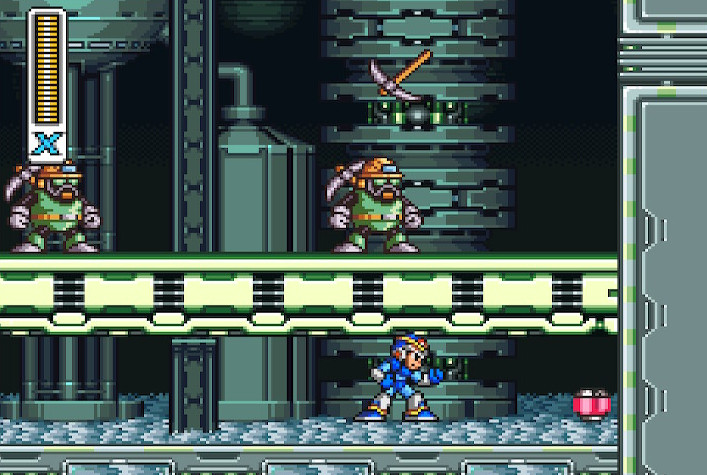
\includegraphics[width=\linewidth]{figures/X1/Flame_heart_2.jpg}
		\caption{}
	\end{subfigure}\\
	\caption{Flame Mammoth's Heart Tank location. To get it defeating Chill Penguin is mandatory.}
\end{figure}

\subsection{Flame Mammoth}\label{boss:Flame_mammoth}
Flame Mammoth, the ``\textit{Blazing Oil Tank}''\cite{book:MMX_Complete_art} was the captain of the 4t Land battalion, with base in the Middle East, before joining Sigma and being labeled as Maverick. His big size and firepower have always been his pride, making him arrogant and cocky, eventually even leading to enjoy bullying/humiliating smaller reploids (which as \cite{wayback:X_resources} states, he even hates), Chill Penguin(\ref{boss:Chill_Penguin})\cite{wiki:Flame_mammoth} included. He's only desire was to show his full power and use it an go into a violent rampage and destroy everything he wants, and Sigma's rebellion was the perfect way to achieve it. However due to being an extremely arrogant and hated leader, no one of his old battalion followed him\cite{MHX:manual}.

The battle against Mammoth takes place in a large arena on top of a conveyor belt Mammoth himself commands. He has three main attacks: When he use his ``Oiling'' he launches a blob of oil (stored in his stomach\cite{wayback:X_resources}) from his trunk. The oil itself does not harm X but can set up a trap when combined with another of Mammoth's attack, the Fire Wave. With this attack, Flame Mammoth shoots several fireballs from his buster towards X which fall onto the ground. If a fireball makes contact with the oil, it bursts into pillar of fire. Finally Mammoth can use his ``Jump Press'' attack, which sees him leaping toward X in order to crush him. Once he lands, a shock-wave is produced which stuns X making him fall onto the ground, if he was on the ground when Mammoth landed. Occasionally Flame Mammoth will also trumpet inverting the direction the conveyor is facing. 

\begin{figure}[h]
	\centering
	\begin{subfigure}{0.4\textwidth}
		\centering
		
\includegraphics[width=\linewidth]{figures/X1/Mammoth_oil.jpg}
		\caption{}
	\end{subfigure}
	\begin{subfigure}{0.4\textwidth}
		\centering
		
\includegraphics[width=\linewidth]{figures/X1/Mammoth_fire.jpg}
		\caption{}
	\end{subfigure}\\
	\begin{subfigure}{0.5\textwidth}
		\centering
		
\includegraphics[width=\linewidth]{figures/X1/Mammoth_oil_fire.jpg}
		\caption{}
	\end{subfigure}
	\begin{subfigure}{0.3\textwidth}
		\centering
		
\includegraphics[width=\linewidth]{figures/X1/Mammoth_trunk.jpg}
		\caption{}
	\end{subfigure}
	\end{figure}

	\begin{figure}
	\ContinuedFloat
	\centering
	\begin{subfigure}{0.4\textwidth}
		\centering
		
\includegraphics[width=\linewidth]{figures/X1/Mammoth_press_1.jpg}
		\caption{}
	\end{subfigure}
	\begin{subfigure}{0.5\textwidth}
		\centering
		
\includegraphics[width=\linewidth]{figures/X1/Mammoth_press_2.jpg}
		\caption{}
	\end{subfigure}
	\caption{Flame Mammoth's attack: (a) Oiling, (b) Fire Wave, (c) Oil ignited by the fire, (d) Trumpet, (e),(f) Jump Press }
\end{figure}

Battling Flame Mammoth can be tricky, but is not impossible. While his oil and Fire Wave attacks are rather simply to dodge, the real threat reside in his press attack, which he will use often and, moreover, he will perform from off-screen. The arena in fact is much wider than all other, not fitting into a single screen. This can lead to the boss to attack from outside the field of view of the player, that has  to act quickly to dodge incoming attacks, such as Mammoth leaping onto X. Furthermore, as stated previously, his jump attack also creates a tremor which stun X if on the ground, so avoid his landing may not be sufficient. Flame Mammoth weakness is the Storm Tornado which however just deals more damage to him and can dispel his flame attack, but it has no other effect on Mammoth himself. What instead has an effect on Flame Mammoth is the boomerang cutter: three hits will cut his trunk, preventing him to spit oil and to reverse the belt direction.

By beating Flame Mammoth X gain the Fire Wave (\ref{Fire_wave}) and, by consequence, the access to Chill Penguin's heart tank (see \ref{Penguin:heart_tank}). However beating this stage has no interaction with others stages.

According to data available, Flame Mammoth is 321 cm tall and 327 Kg heavy (slightly heavier than what portrayed in game).

\begin{figure}[h]
	\centering
	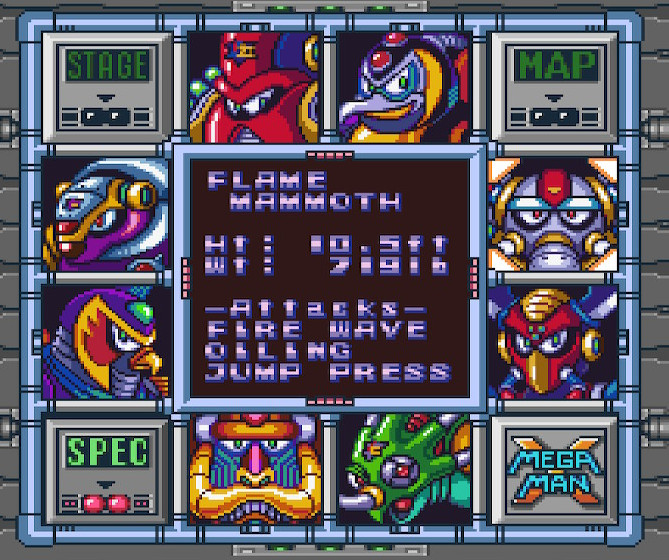
\includegraphics[width=0.5\linewidth]{figures/X1/Flame_mammoth_specs.jpg}
	\caption{Flame Mammoth specifications according to X1.}
\end{figure}
\section{Airport}
In the \textit{Airport stage} (or \textit{New Type Airport} in the remake) X starts from the ground and has to climb up the airport structures in order to reach the Death Rogurmer as it leaves, in order to destroy it. 

The stage focus mainly on platforming above bottomless pit and on moving platforms, as it takes place in the sky. Various enemies are also placed on some of this platform in order to obstacle X while jumping. X starts on the ground and has immediately to climb using some moving platforms to reach the airport's roof, while some \hyperlink{enem:Sky_Claw}{Sky Claws} try to grub him and make him fall into the pit. After reaching the roof, X can either continue along it, fighting more enemies while going, or can destroy the lift cannon at the beginning , and use the platform it leaves behind to reach the top of the nearby tower, where X can enter after destroying the window and go through, skipping below enemies. Next is a platforming section with a series of platform which move up and down in an alternate way. Furthermore on some of them \hyperlink{enem:Flamer}{Flamers} are positioned, which have a good horizontal range and must destroyed in order for X to step on the platform. However they are positioned every other platform, meaning the player can skip them, by dash-jumping from the platform X stands when it's at the peak (meaning the next one with the enemy is lower) and landing two platforms ahead, in an empty one. Following this part, there is a pretty straightforward section where X has to defeat more enemies in order to proceed. Finally the last part begins with a series of three platforms above a bottomless pit which will proceed to fall as X steps on them, giving the player few time to jump onto the following one. Passed this X will reach the Death Rogumer itself and, after passing its two cannons, X will stand in front of the boss door. On the far right of the ship, before entering the boss, a weapon tank and a health tank are present onto the ship wing.

The stage has the following enemies\cite{wiki:Airport}:
\begin{itemize}
	\item \hyperlink{enem:Ball_De_Voux}{Ball De Voux }
	\item \hyperlink{enem:Flamer}{Flamer}
	\item \hyperlink{enem:Gun_Volt}{Gun Volt}
	\item \hyperlink{enem:Hoganmer}{Hoganmer}
	\item \hyperlink{enem:Lift Cannon}{Lift Cannon}
	\item \hyperlink{enem:Metall_C-15}{Metall C-15}
	\item \hyperlink{enem:Sky_Claw}{Sky Claw}
	\item \hyperlink{veichle:Death Rogumer}{Death Rogumer}'s cannons
\end{itemize}

\subsection{Heart Tank}
Right at the beginning of the stage, if when the rising platform reaches its top X jumps left instead of right will land onto a platform right above the starting point but not accessible from below. On this platform is where the Heart Tank is.
\begin{figure}[h]
	\centering
	\begin{subfigure}{0.4\linewidth}
		\centering
		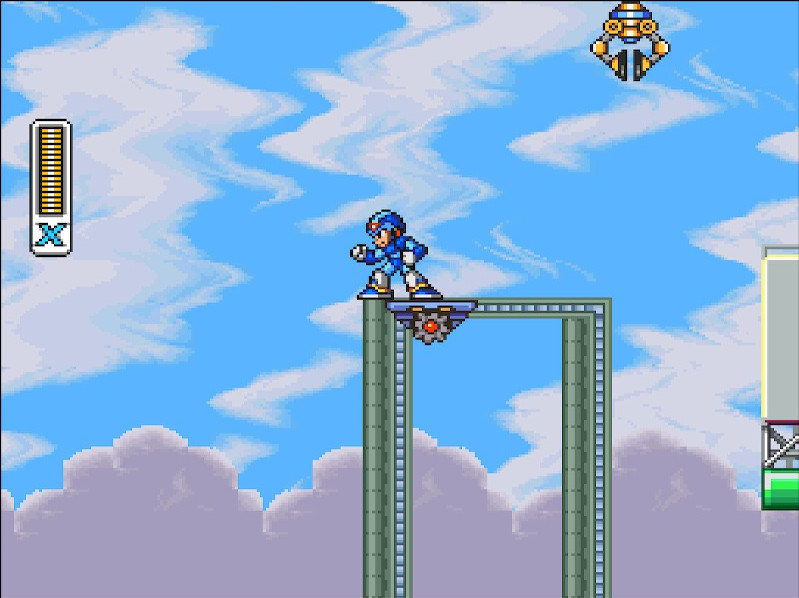
\includegraphics[width=\linewidth]{figures/X1/Storm_heart_1.jpg}
		\caption{}
	\end{subfigure}
	\begin{subfigure}{0.4\linewidth}
		\centering
		
\includegraphics[width=\linewidth]{figures/X1/Storm_heart_2.jpg}
		\caption{}
	\end{subfigure}
	\caption{Airport's Heart Tank location. A dash-jump from (a) to the left bring the player to the Heart's location (b).}
\end{figure}

\subsection{Sub Tank}
After reaching the Airport roof the player will find a 	\hyperlink{enem:Lift_cannon}{Lift Cannon}, a cannon on top of a platform which will rise and lower as the cannon spins. Once destroyed the cannon the platform will fall down, only to rise again as X stands on it, to bring him near a window X can destroy and enter the tower. Here a \hyperlink{enem:Gun_Volt}{Gun Volt} is present and, as X destroys it, all windows will shatter, opening and exit on the opposite side X has entered. At the end of the tower is where the Sub Tank is. 
 
 \begin{figure}[h]
 	\centering
 	\begin{subfigure}{0.4\linewidth}
 		\centering
 		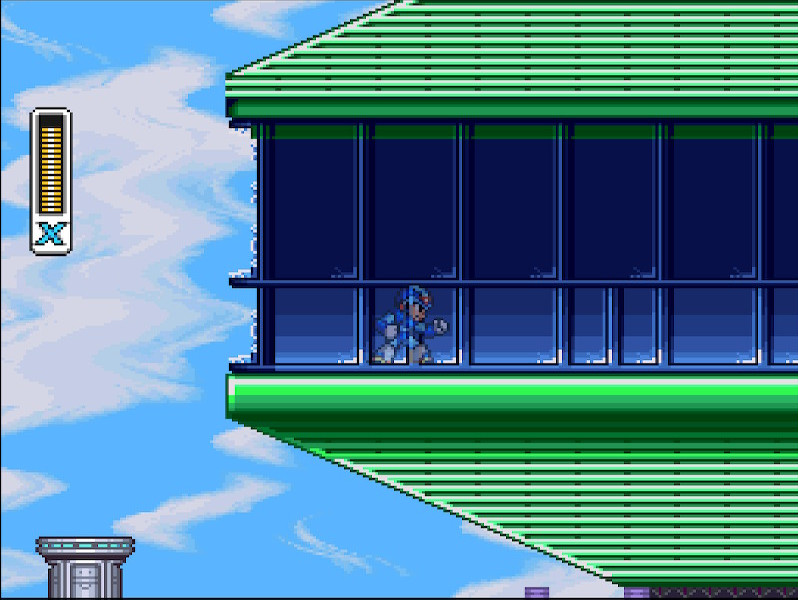
\includegraphics[width=\linewidth]{figures/X1/Storm_tank_1.jpg}
 		\caption{}
 	\end{subfigure}
 	\begin{subfigure}{0.4\linewidth}
 		\centering
 		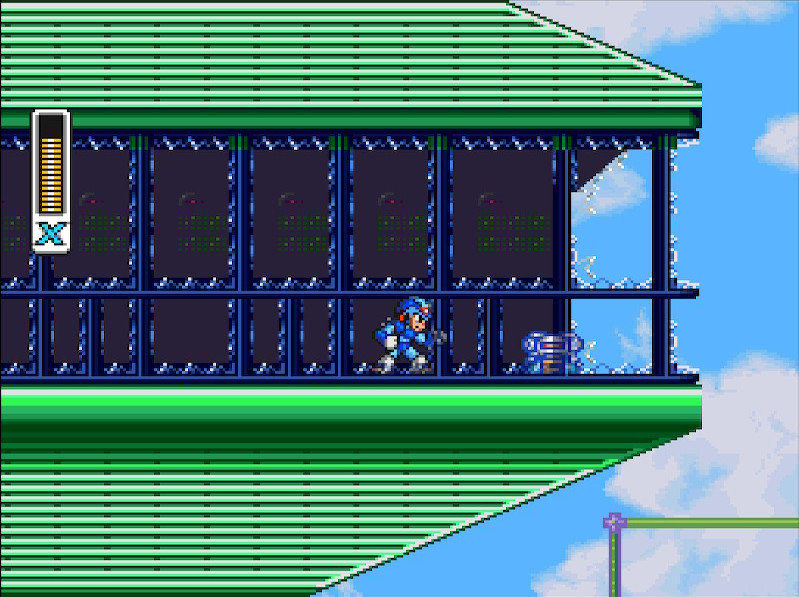
\includegraphics[width=\linewidth]{figures/X1/Storm_tank_2.jpg}
 		\caption{}
 	\end{subfigure}
 	\caption{Airport's Sub Tank location. From the top of the platform X has to break the window (a) and enter the tower. At the end (b) is where the Sub Tank is.}
 \end{figure}
 
\subsection{Head Parts} 
 While traveling the stage the player may notice that in some locations there are canisters bearing a flammable mark onto them. While it is logical to think the Fire Wave weapon is necessary to detonate them, this is not true and X buster's charged shots can work as well, only requiring few more shots. While most of them only hide health tanks or life up, the one near the pylon after the sequence with moving platforms hides a secret path which leads to the Head Parts. 
 
 \begin{figure}[h]
 	\centering
 	\begin{subfigure}{0.4\linewidth}
 		\centering
 		
\includegraphics[width=\linewidth]{figures/X1/Storm_armor_1.jpg}
 		\caption{}
 	\end{subfigure}
 	\begin{subfigure}{0.4\linewidth}
 		\centering
 		
\includegraphics[width=\linewidth]{figures/X1/Storm_armor_2.jpg}
 		\caption{}
 	\end{subfigure}
 	\caption{Head part location: by destroying the fuel tanks the capsule is on the right.}
 \end{figure}
 
 \subsection{Storm Eagle}\label{boss:Storm_Eagle}
 Storm Eagle was the taciturn, calm, careful strategist and leader of the Maverick Hunters' 7th Airborne Unit\cite{wiki:Storm_Eagle}. Although not talking much and being difficult to approach, Storm Eagle was a very popular leader among his men\cite{MHX:manual}. Loyal to his job as Maverick Haunter, when the rebellion broke out Eagle's first reaction was to haunt down and challenge Sigma. However Sigma was no match for him, and Storm Eagle was forced to surrender. It not clear however if him joining Sigma was mostly due simply to an self-preservation instinct (as the original game and the collection hint\cite{Xcoll1:Manual_X1}) or due his pride, which forced him to follow Sigma even if reluctant (hinted in remake). In both cases Storm Eagle ended up controlling the Death Rogumer, a new type of aerial battleship (the same one X meets at the end of the Highway Stage from which Vile descends).
 
 
 \begin{figure}[h]
 	\centering
 	\begin{subfigure}{0.3\linewidth}
 		\centering
 		
\includegraphics[width=\linewidth]{figures/X1/Eagle_egg_1.jpg}
 		\caption{}
 	\end{subfigure}
 	\begin{subfigure}{0.35\linewidth}
 		\centering
 		
\includegraphics[width=\linewidth]{figures/X1/Eagle_egg_2.jpg}
 		\caption{}
 	\end{subfigure}\\
	 \begin{subfigure}{0.4\linewidth}
	 	\centering
	 	
\includegraphics[width=\linewidth]{figures/X1/Eagle_push.jpg}
	 	\caption{}
	 \end{subfigure}
	 \begin{subfigure}{0.4\linewidth}
	 	\centering
	 	
\includegraphics[width=\linewidth]{figures/X1/Eagle_tornado.jpg}
	 	\caption{}
	 \end{subfigure}\\
 		 \begin{subfigure}{0.4\linewidth}
 		\centering
 		\includegraphics[width=\linewidth]{figures/X1/Eagle_dive.jpg}
 		\caption{}
 	\end{subfigure}
 	\caption{Storm Eagle attacks: (a),(b) Bird Summon, (c) Gust, (d) Storm Tornado and (e) Dive.}
 \end{figure}
 
 The difficulty of the battle against Storm Eagle can vary a lot depending on whether X has already obtained the Foot Parts(\ref{X:Foot_Parts}). This is due the fact that most of Storm Eagle's attacks (two out of four) revolve around pushing X off the arena (which is only a long platform onto of a pit with no walls) and the dash completely nullify these attacks. In particular these two attack are his Gust\cite{wiki:Storm_Eagle} and Storm Tornado. The former sees Eagle flapping his wings to create a rush of air which push X away at a slow rate and simply walking can prevent X from falling, if he has enough space left, while the latter generates a horizontal tornado which doesn't deal any damage but push X much faster and, without dashing through, can be hard to counter. Next Storm Eagle has his Diving attack, that makes him rise out of the screen to dive-bomb diagonally onto X several times before returning on the ground. X can either focus on dodging Eagle, which should be rather simple as the arena is enough tall and wide to see Eagle diving in advance, or can even try to hit him, as he's not invincible while performing this attack. Finally Storm Eagle has his Bird Summon attack, that consists in him shooting out an egg from his beak while hovering mid-air and, if the egg hits the ground, it hatches into four mini bird-like robots which fly towards X. Storm Eagle's weakness is the Chameleon Sting which deals him more damage and, thanks to its angle, can hit him better when he's mid-air. Upon defeating him, X will gain the Storm Tornado\ref{Storm_tornado} and, furthermore, the Death Rogumer will crash land onto the Power Plant Stage cutting the electricity in some section, making the level easier to navigate (moreover the the airship will also disappear from the map screen).
 
 Storm Eagle is 250 cm tall and 135 Kg heavy, while his title is ``\textit{Nobleman of the Skies}''\cite{book:MMX_Complete_art}.
 
 \begin{figure}[h]
 	\centering
 	\includegraphics[width=0.5\linewidth]{figures/X1/Storm_eagle_specs.png}
 	\caption{Storm Eagle specifications according to X1.}
 \end{figure}
\section{Tower}
Among all other stages, the \textit{Tower Stage} (or \textit{Fortress Tower}) is the most different due the fact of extending mostly in vertical. This translate in the player having to climb it via wall-jumping or using moving platforms, with the risk of being hit and fall down at the beginning.

The first part of the stage sees X climbing a series of platform placed in a zig-zag patter and with enemies on them, which will try to attack X while jumping from one to another and make him fall down. Next is a horizontal section in which \hyperlink{enem:Sine_Faller}{Sine Faller} will keep spawning and chasing after X which will have also to deal with laser traps, which will shoot X if he passes trough triggers while active. The traps cannot be destroyed, but it is possible to trigger them and avoid lasers if the player move fast enough. 

The next part is pretty straightforward: it is another vertical section divided into different levels, one on top of another, each one with a \hyperlink{enem:Mega_Tortoise}{Mega Tortoise} in the center which will shoot bombs at X's position. These enemies cover are placed on top of platforms and, due their size, make difficult to proceed undamaged without disposing of them first (although it is still possible by precise dash-jumps). Once on top the player will reach an elevator with spikes all along the walls. As X stands on it, it will start ascending. While rising the elevator will go towards some platform with spike beneath them, which will insta-kill X if he isn't fast enough to dodge them. Furthermore other enemies will spawn and aim at X to obstacle his movements. As the elevator goes up it will start increasing its speed making more difficult to avoid obstacles. Near the end of its ride the elevator will slow down to let X dismount in time, before crashing against the spiked roof. During this part a trick can be performed: if X stands on the rightmost side of the elevator he will avoid all spiked platform, eliminating the major risk factor of this part (see fig. \ref{tower_spike} or the video file \texttt{Tower\_spike\_skip.mp4} for more information). Next there are two other climbing sections, one on the outside with moving platform and enemies on top of them, and the last one, inside, again with enemies on top of moving platform and on walls as well. At the end of this last part the player will find the boss door.
\begin{figure}[htp]
	\centering
	\includegraphics[width=0.5\linewidth]{figures/X1/Tower_spike_skip.jpg}
	\caption{By standing in this precise position X will not collide with any spikes, even the lateral one, lowering the difficulty of this section.}
	\label{tower_spike}
\end{figure}


This stage contains following enemies\cite{wiki:Tower}:

\begin{itemize}
	\item \hyperlink{enem:Dodge_Blaster}{Dodge Blaster}
	\item \hyperlink{enem:Hoganmer}{Hoganmer}
	\item \hyperlink{enem:Jamminger}{Jamminger}
	\item \hyperlink{enem:Ladder_Yadder}{Ladder Yadder}
	\item \hyperlink{enem:Mega_Tortoise}{Mega Tortoise}
	\item \hyperlink{enem:Sine_Faller}{Sine Faller}
	\item \hyperlink{enem:Slide_Cannon}{Slide Cannon}
	\item \hyperlink{enem:Turn_Cannon}{Turn Cannon}
\end{itemize}

\subsection{Heart Tank}
This stage's Heart tank is hidden in plain sight, right at the end of the outside section,on a large platform near the entrance for the last stage's portion. While being easy to spot, is isn't as easy to get, especially during the stage's first run. Three methods exists to get it. The first and easiest way is to replay the stage after having acquired the Boomerang Cutter and use a boomerang to grub it from the tower's inside, since boomerangs pass trough wall. The second way is to use a charged Shotgun Ice from the entrance and ride the platform while midair, to perform a dash jump from it which will give X enough high to grub to the platform's edge (see video file \texttt{kuwanger\_heart\_ice.mp4}). Finally it is also possible to reach the platform via a pixel-perfect dash-jump which gives X barely enough high to trigger a wall-jump of the platform's edge and subsequently reach its top and the Heart Tank (see \ref{X1:misc} for information on involved tricks). This last technique is known as \textit{Iceless}. 
\begin{figure}[htp]
	\centering
	\includegraphics[width=0.5\linewidth]{figures/X1/Tower_heart.jpg}
	\caption{Tower Stage's Heart Tank location.}
\end{figure}


\subsection{Boomer Kuwanger}\label{boss:Boomerang_Kuwanger}
Boomer Kuwanger (lately renamed \emph{Boomerang} Kuwanger) was a former Maverick Haunter of the 17th Elite Unit under the direct command of Sigma (and also partner of X and Zero in the \mhx remake). However due to his cold, analytic, almost nihilist\cite{book:MH_field_guide}, and cynical vision of the world, he has never had a true sense of justice nor ideals, acting only following logic and his own interest\cite{MHX:manual}. This has lead him to join Sigma's rebellion without interest in its meanings, but the true reasons of his choice has never been explained. Some sources suggest Kuwanger went Maverick and followed Sigma only has it was the most logical action\cite{MHX:manual}, due to his own interest\cite{wiki:Boomer_kuwanger} or even both\cite{book:MH_field_guide}. Other sources even suggest he went Maverick out of fun\cite{Xcoll1:Manual_X1} or out of spite for humans\cite{wayback:X_resources}. Whatever Boomer Kuwanger's reasons were, after joining Sigma he conquered the tower symbol of the city, to convert it into his own base.

In battle Boomer Kuwanger attack with his signature ability, the instant transmission, which allow him to teleport across the arena, typically behind his opponent, to strike him with his horns. This teleportation ability worth him the title of  ``\textit{Blade Demon of Space and Time}''\cite{book:MMX_Complete_art}. Once Kuwanger reappears he will perform one attack between Boomerang Cutter and Death Lift. With the first one he will throw his horns toward X with a curved trajectory which will then travel back to him, as the name suggest, while when performing the second one, Death Lift, he will grub X with his mandibles and throw him into the ceiling dealing large damage. Finally Boomer Kuwanger also has a dash attack, where he dash toward X to damage him.
 \begin{figure}[htp]
	\centering
	\begin{subfigure}{0.4\linewidth}
		\centering
		\includegraphics[width=\linewidth]{figures/X1/Boomer_lift_1.jpg}
		\caption{}
	\end{subfigure}
	\begin{subfigure}{0.3\linewidth}
		\centering
		\includegraphics[width=\linewidth]{figures/X1/Boomer_lift_2.jpg}
		\caption{}
	\end{subfigure}\\
	\begin{subfigure}{0.4\linewidth}
		\centering
		\includegraphics[width=\linewidth]{figures/X1/Boomer_dash.jpg}
		\caption{}
	\end{subfigure}
	\begin{subfigure}{0.4\linewidth}
		\centering
		\includegraphics[width=\linewidth]{figures/X1/Boomer_throw.jpg}
		\caption{}
	\end{subfigure}
	\caption{Boomer Kuwanger attacks: (a),(b) Death Lift, (c) Dash and (d) Boomerang Cutter.}
\end{figure}
Dealing with Boomer Kuwanger isn't easy without his weakness, as the continuous teleporting makes him hard to hit with buster shots more than once. Furthermore the player has to keep moving in the arena to avoid Kuwanger to teleport near him and use his Death Lift attack for massive damage.

The boss fight takes a turn when fought with Boomer Kuwanger main weakness: the Homing Torpedo (\ref{Homing_torpedo}). Since missiles shot with this weapons lock onto enemies they can chase Kuwanger even when teleporting, meaning they will always hit him no matter his position. This drastically reduce the fight complexity as X can literally hide in a corner while shooting torpedoes which will automatically hit Boomer Kuwanger, also with increased damage as they're his weakness.

According to his specifications Boomer Kuwanger is 242 cm tall and 94 Kg heavy (again, different from in-game information which makes him shorter and lighter). More interesting however is the fact Boomer Kuwanger is one of few reploids known to have family relationship with another reploid (in this specific case a brother): Gravity Beetle.%\ref{Gravity_beetle}.

After defeating him X will gain the Boomerang Cutter weapon(\ref{Boomerang_cutter}) for his own use.
\begin{figure}[htp]
	\centering
	\includegraphics[width=0.5\linewidth]{figures/X1/Boomer_kuwanger_specs.png}
	\caption{Boomer Kuwanger in-game specs.}
\end{figure}

\section{Power Plant}
The \textit{Power Plant} (or \textit{Electromagnetic Power Plant} in the remake) stage is where Spark Mandrill resides. As to be expected from its name, this stage's main feature revolve around electricity in various form. However if the player manages to defeat Storm Eagle first the Death Rogumer will crash land onto this stage, cutting the power and removing part of the stage's hazards. 
The first section of the stage consists in a maze of pipes split into different levels connected by ladders. Here, along with some enemies, electric sparks will spawn and travel along the ground, dealing damage on contact. Passed this part a dangerous one awaits: here the light will shut down at regular interval making difficult to spot the level layout, especially pits. Furthermore along the stage  \hyperlink{enem:Hotarion}{Hotarions} will spawn traveling horizontally while also illuminating the stage along their path. They can be rather dangerous as the move fast and, if the player doesn't know where they spawn, can hit X while jumping and make him fall into a pit.
At the middle of the stage a sub-boss is present: the \hyperlink{miniboss:Thunder_slimer}{Thunder Slimer}. Its main attack consists in leap into X with his big hitbox or to block X by scattering round bubbles of slime which trap X in place, making him vulnerable to his lightning bolts which it will shoot after having absorbed electricity from the plant. If the player has cut off the power Thunder Slimer will no be able to perform this last attack.

Passed the sub-boss there is a more traditional section with enemies placed along the way which ends with another platforming part with light going off. Once passed this section the player will reach the boss room.

Following enemies appear in this stage\cite{wiki:Power_plant}:
\begin{itemize}
	\item \hyperlink{enem:Ball_De_Voux}{Ball De Voux}
	\item \hyperlink{enem:Flammingle}{Flammingle}
	\item \hyperlink{enem:Jamminger}{Jamminger}
	\item \hyperlink{enem:Gun_Volt}{Gun Volt}
	\item \hyperlink{enem:Hotarion}{Hotarion}
	\item \hyperlink{enem:Mega_Tortoise}{Mega Tortoise}
	\item \hyperlink{enem:Rush_Roader}{Rush Roader}
	\item \hyperlink{miniboss:Thunder_Slimer}{Thunder Slimer}
	\item \hyperlink{enem:Turn_Cannon}{Turn Cannon}
\end{itemize}


 


\subsection{Sub Tank}
This stage's Sub Tank can be found right at the beginning of the stage in the tube ``maze''. It is however unreachable since the room where it is has no entrance. This force the player to use the Boomeran Cutter's ability to grub item from distance in order to get it.

\subsection{Heart Tank}
While not properly hidden, this stage Heart Tank can be easily missed if the player does not pay enough attention during the level. More in detail, the Heart Tank is hidden at the end of the corridor passed Thunder Slimer, before descending the ladder. It is placed in the rightmost corner, which players could easily avoid if they fall down immediately instead of climbing the wall.

In order to get the collectible two option are possibles: by using again Boomerang Cutter's grub ability or with a accurate dash-jump from the wall.

\subsection{Spark Mandrill}\label{boss:Spark_mandrill}
Spark Mandrill was originally a Maverick Haunter of the 17th Elite unit directly under Sigma control. When the latter started his revolt, Mandrill followed his commander without questioning, thus being labeled as a Maverick. While not being very smart he compensated in raw power\cite{MHX:manual} which, also due his taste for electricity, made him the perfect candidate to seize the Power Plat, to private cities of electric power while also granting Sigma an energy source. Another main trait Mandrill was also know for was his laziness. In fact once seized the Power Plant, he left the remaining work to his subordinates, while he stayed in the sidelines napping and chowing of the electricity produced by the main generator\cite{wayback:X_resources}.

Better known as the ``\textit{Quick-Fisted King of Lightning}'' Mandrill keeps faith to his title by fights against X mostly using melee attacks, but he can also use ranged attack in the form of his own Electric Spark whether the situation requires.

Although his size, Mandrill can move quite fast, especially when using his punch attack which comes into two possible ways\cite{wiki:Spark_mandrill}: if X is near Mandrill he will straight hit him with a quick attack which can be hard to dodge due the close distance; meanwhile if the player is far from him, Mandrill while dash toward him while punching. This latter attack is easier to avoid since Mandrill's dash speed is relatively low, hence avoidable.  As said before Spark Mandrill can also attack from the distance using his Electric Spark. With this move Mandrill will punch the ground producing two orbs made of electricity which will travel in split directions along the ground and also along walls. These orbs move relatively fast but can be avoided with a jump at the right timing. Finally Mandrill will sometimes jump and hang to the ceiling and move toward X. When he passes below him, Mandrill will drop down trying to hit him. 

According to his specifications Spark Mandrill is 305cm tall and weights 394 Kg (slightly heavier than in-game information). Upon defeated X will gain the Electric Spark(\ref{Electric_spark}) weapon.
\section{Forest}
Last but not least of \x's main stages is the Forest (or Recon Base Ruins). This is a rather plain and straightforward level with no particular gimmicks involved or secret paths. Finally this is also one of the few stages which change depending if another boss has been defeated before: in this particular case if Launch Octopus is gone the Forest will be flooded. However this doesn't have an impact on the difficulty level, in opposite of other stages with this feature.

The beginning of the level sees X teleporting in the middle of the forest. From here he must proceed to the right fighting enemies, some of them also disguised as bushes, until he reaches the entrance of a tunnel. From here there are three possible paths: if X climbs the wall above the tunnel he will reach and area with the optional miniboss \hyperlink{miniboss:RT-55J}{RT-55J} and the Armor Parts; if he slide down the pit he will reach a hidden cave with the Heart Tank; finally if he proceed straight he will go on in the stage. While in the tunnel an earthquake will cause rocks to fall from the roof, damaging X if they hit him. Moreover enemies will also fall from the roof: they're \hyperlink{enem:Crag_man}{Crag Men} which disguise themselves as rocks and fall onto X as he passes beneath, only to transform after hitting the floor. This section is far less dangerous if X has either defeated RT-55J (which was the earthquake's cause) or obtained the helmet parts (which makes X invulnerable to falling rocks). In both cases Crag Men will always be present.

The last portion of the Stage is a Ride Armor section. Right at the beginning X is given a Ride Armor to proceed in the stage, which now present large ponds of mud which makes X and the Armor slowly sink, interrupted by small platform where the player can stand on. While X can free himself by repeatedly jumping, one the Ride Armor sinks it is gone. This can be problematic since near the end enemies Ride Armors will start attacking and can be tough to take down without using one too. At the end of this stage's portion the player will find the boss door.

Following enemies appear in this stage\cite{wiki:Forest}:
\begin{itemize}
	\item \hyperlink {miniboss:RT-55J}{RT-55J}
	\item \hyperlink {enem:Amenhopper} {Amenhopper}
	\item \hyperlink {enem:Armor_Soldier} {Armor Soldier(with Ride Armor)}
	\item \hyperlink {enem:Axe_Max} {Axe Max}
	\item \hyperlink {enem:Crag_Man} {Crag Man}
	\item \hyperlink {enem:Creeper} {Creeper}
	\item \hyperlink {enem:Hoganmer} {Hoganmer}
	\item \hyperlink {enem:Jamminger} {Jamminger}
	\item \hyperlink {enem:Mad_Pecker} {Mad Pecker}
	\item \hyperlink {enem:Planty_Iworms} {Planty\&Iworms}
\end{itemize}

\subsection{Armor Parts}
The armor parts is found near the beginning of the stage, before entering the tunnel. If X climbs the wall above said tunnel (reachingit by a dash-hump from above the pit) and proceed right he will reach an arena which will immediately close the exit with some falling rocks, and the RT-55J miniboss will spawn. His main attacks consists using his claw to grub X (or pull itself towards the wall if the claw hits it) or, if X is out of the claw's range, jump onto him. Its weak point are the head and his hole body, which however is covered most of the times by its claw, which is instead immune to all attack. This means that beside specific occasions (such when it throws the claw), the main spot to hid is the head. Due the lack of invincibility frames, the Storm Tornado is the best choice, although the Boomerang Cutter is considered its main weakness\cite{wiki:RT55J}. As the fight proceed RT-55J will start smoking, hinting the fact that his health bar is low. Once the miniboss has been defeated the Light Capsule with the enhancement will rise from the ground.

\subsection{Heart Tank}
The Heart Tank position is mirrored respect the Armor Parts. To reach it X has in fact to slide down the pit near the beginning of the stage to find a wall breakable by the Foot Parts which leads to a small cavern. Once inside the Heart Tank will be on a small platform in the top-right corner of the room, above a bottomless pit. X cannot reach it normally with dash jump due the distance, but he can if  the cave is flooded as consequence of defeating Launch Octopus\ref{boss:Launch_octopus}, thanks to the extra height X gains when jumping underwater. Doing a wall dash-jump from the cave entrance is not recommended, since X will hit the roof and fall.

\subsection{Sting Chameleon}\label{boss:Sting_chameleon}
Sting Chameleon once belonged to the Maverick Haunter Ranger Unit (namely 9th Special Force\cite{wayback:X_resources}) He was a very high-Haunter which however was never worth a promotion due his sly ,sneaky and sharp-tongue nature, which made him unpopular\cite{Xcoll1:Manual_X1} among his commander or other members of his unit. Furthermore Chameleon's preference for strategy and his strong belief in the ``\textit{By any mean necessary}'' mantra  worth him the title of coward\cite{MHX:manual}. Once Sigma started his riot, Chameleon saw an opening to rise through ranks and prove what he capable of. Sigma then proceed to put him in charge of defending the front-line base in the forest.

Sting Chameleon uses three main weapons when fighting\cite{wiki:Sting_chameleon}: his natural ability to blend with the surrounding, which makes him almost invisible to enemies, his long tongue, which he use to deliver high-speed attacks or even to hang himself around, and his main projectile, the Chameleon Sting, which he shots from his tail. These weapons all translate in attack he can perform while battling X at the end of the Forest Stage. His main method of movement is his Transparent Movement, which makes him transparent and invincible. After a short amount of time Chameleon will reappear, usually hanged on the background, ready to attack X. The player can however spot his position as the distortion he causes when moving, and intercept him before he launches his attack. If Chameleon reappears near X this means he will use his Iron Tongue attack, which strikes the player by rapidly extending his tongue, even up to three times in a row. Otherwise if he reappears in a top corner, then he will use his Chameleon Sting attack, shooting a sheet of projectile by swinging his tail. Finally Chameleon can also hang to the roof by using his tongue and start shaking, causing spikes to fall from the roof (Thorn Rain) which will damage X, even with the Helmet Parts equipped.

While fighting Sting Chameleon without the correct weapon is not trivial, everything changes when using the Boomerang Cutter, his weakness. Although at first it seems this weapons only does increased damage to him, since it does not sever him like Flame Mammoth or Launch Octopus, at a more accurate analysis is possible to see this weapon force his AI into a loop which can be exploited to end the fight quickly. Once hit Chameleon will, in fact, always move to the opposite side of the room and use his Thorn Rain attack. This means that the only thing the player has to do is stay in the center of the room, shooting some Boomerang Cutters where Chameleon will reappears and, as soon as he gets hit, turn and do the same thing in the opposite direction. The player hasn't even to take care of weapon energy, as all boomerangs which don't hit the boss will return replenishing the weapon energy. 

According to data Sting Chameleon was 177 cm tall and 77 Kg heavy, while his title was ``\textit{Frightening Forest's Strike}''
After defeating Sting Chameleon X will add the Chameleon Sting(\ref{Chameleon_sting}) weapon to his arsenal.

\section{Sigma Stage (1-4)}
\section{Miscellaneous}\label{X1:misc} %wall clip glithc, seven pixel, auto edge grub flying hadoken %subt-tank + life farming